\chapter{KernelShark}
\label{kap-kernel-shark}

Tato kapitola pojednává o programu KernelShark, což je GUI program pro vizualizaci a analýzu trasovacích dat z programu Trace-cmd. Kapitola nejprve krátce představí jeho autory, přispěvatele a účel. Dále se bude zabývat tím, jak KernelShark používat a jeho pluginy. Nakonec kapitola načrtne architekturu KernelSharku v modulech. Často budeme čerpat ze stránek KernelSharku \cite{KernelShark-Pages}.

\section{O autorech}

KernelShark začal být vyvíjen v roce 2009 Stevenem Rostedtem jako GUI frontend pro data z Trace-cmd. Steven Rostedt je velkým přispěvatelem do Linuxového jádra, hlavně co se týče trasování, a udržuje repozitář pro Trace-cmd, jímž je také autorem. Dnes je zaměstnancem Googlu\footnote{\citetitle{SR-LinkedIn} \cite{SR-LinkedIn}}, dříve ale pracoval ve známých společnostech jako Red Hat nebo VMWare. V článku \cite{LWM-Kshark} pak na této verzi KernelSharku ukázal analýzu plánovače úloh v reálném čase a zároveň představil funkcionality svého programu, například filtrování událostí podle procesu či plovoucí okénko s informacemi o vybrané události. KernelShark se nadále vyvíjel a k projektu se v roce 2017 (dle dat commitů v repozitáři) oficiálně přidal Yordan Karadzhov. Vystudovaný částicový fyzik, Yordan Karadzhov se později zaměřil na vývoj software a dnes pracuje u firmy Bosch jako softwarový inženýr\footnote{\citetitle{YK-LinkedIn} \cite{YK-LinkedIn}} a je dnes nejvýraznějším přispěvatelem do KernelSharku.

Projekt je open-source a přispěvatelé pak žádají vlastníky repozitáře o publikaci svých commitů. Ke dni psaní je nejnověší dostupnou verzí \texttt{2.4.0}.

\section{Instalace}

Program nabízí někteří existujícící manažeři software na různých distribucích, například Zypper na openSUSE nebo Apt na Ubuntu. K dispozici je také balíček pro vývoj. Program si lze i stáhnout jako tarball a instalovat jej ručně. Poslední možností je klon gitového repozitáře, který si sami sestavíme. Manažeři závislosti a instalaci vyřeší za nás, proto zbytek této sekce se bude zajímat hlavně o ruční sestavení programu.

\subsection*{Předpoklady k instalaci}

K sestavení je nutné mít na systém překladač pro jazyky C a C++ a sestavovací systémy Make a CMake. KernelShark je grafický program a k tomu využívá framework Qt, specificky Qt6. Dalšími grafickými nutnostmi jsou vývojové soubory pro FreeGLUT3 a vývojové soubory pro knihovny libXmu a libXi. KernelShark využívá pro některé své funkcionality soubory ve formátu JSON a je zapotřebí mít k dispozici knihovnu \texttt{libjson-c}. Potřebný je i textový font FreeSans, který může být nalezen v různých balíčcích dle distribuce (\texttt{fonts-freefont-ttf} na Ubuntu a \texttt{gnu-free-sans-fonts} na Fedoře). Jako frontend pro Trace-cmd nakonec vyžaduje přítomnost tohoto programu a knihoven \texttt{libtracefs} a \texttt{libtraceevent}. Zbylými nutnými závislostmi jsou Flex a Bison. Volitelnými závislostmi jsou pak Doxygen a Graphviz, které slouží ke generování dokumentace.

Abychom byli schopni využít KernelShark naplno, je také nutné pracovat v prostředí, kde fungují Polkity. Těmi může KernelShark požádat o dočasný superuživatelský přístup pro spuštění Trace-cmd. Autorovi práce program fungoval perfektně v desktopovém prostředí KDE Plasma, nicméně v prostředí Qtile či při práci v Linuxovém subsystému ve Windows byly Polkity pouze napůl funkční, ačkoliv zbytek GUI fungoval bez problému. Problém byl vyřešen automatickým přijetím žádosti o zvýšení práv v pravidlech Polkitů. Tento způsob ale není doporučen, jelikož představuje bezpečnostní riziko.

\subsection*{Sestavení}

Když máme všechny závislosti a zdrojový kód k dipozici, můžeme konečně vybudovat KernelShark. K dispozici máme z typů \emph{Debug}, \emph{Release}, \emph{RelWithDebInfo} a \emph{Package}. Poslední slouží hlavně pro vydavatele balíčků, pokud chtějí KernelShark nějak přesněji přeložit pro daný systém. S výběrem typu sestavení a, volitelně, vytvořením dokumentace, nám pak stačí přsunout se do \texttt{build} adresáře. Z něj pak zavoláme CMake, Make a nakonec jako superuživatel spustíme instalační skript pro GUI. Můžeme také spustit instalační skript pro vytvoření vývojových souborů. KernelShark je odteď sestaven a nainstalován. Knihovny nalezneme v podadresáři \texttt{libs} instalačního adresáře a vytvořené spustitelné binární soubory v podadresáři \texttt{bin}.

\subsection*{Odstranění programu}

Pokud si přejeme KernelShark ze systému odstranit, jsou k dispozici skripty \texttt{cmake\_clean.sh} a \texttt{cmake\_uninstall.sh} v \texttt{build} adresáři.

\section{Použití}

Program lze spustit přes příkazovou řádku. KernelSharku lze při spouštění dodat různé argumenty, například cestu ke specifickému souboru k otevření, nebo pluginy, které se mají načíst.

KernelShark dokáže vizualizovat data z několika souborů naráz, přičemž každý vytváří vlastní datový proud, tj. \emph{stream}, ve kterém jsou data uchována. Pokud uživatel otevře jeden stream, může pak připojovat další streamy. KernelShark zobrazí data ve vlastní skupině grafů pro tento stream a zařadí je na časovou osu, kterou případně rozšíří. Streamy není možné odebírat, jedinou možností pro odebrání streamů je buď restart KernelSharku, či otevření jednoho nového souboru s trasovacími daty. Streamy nemusí být něčím spojené, je možné i otevřít dva streamy z odlišných strojů s různými uálostmi a jinými časovými stopami. Na obrázku \ref{kshark-empty} je čerstvě spuštěný KernelShark.

\begin{figure}[p]\centering
    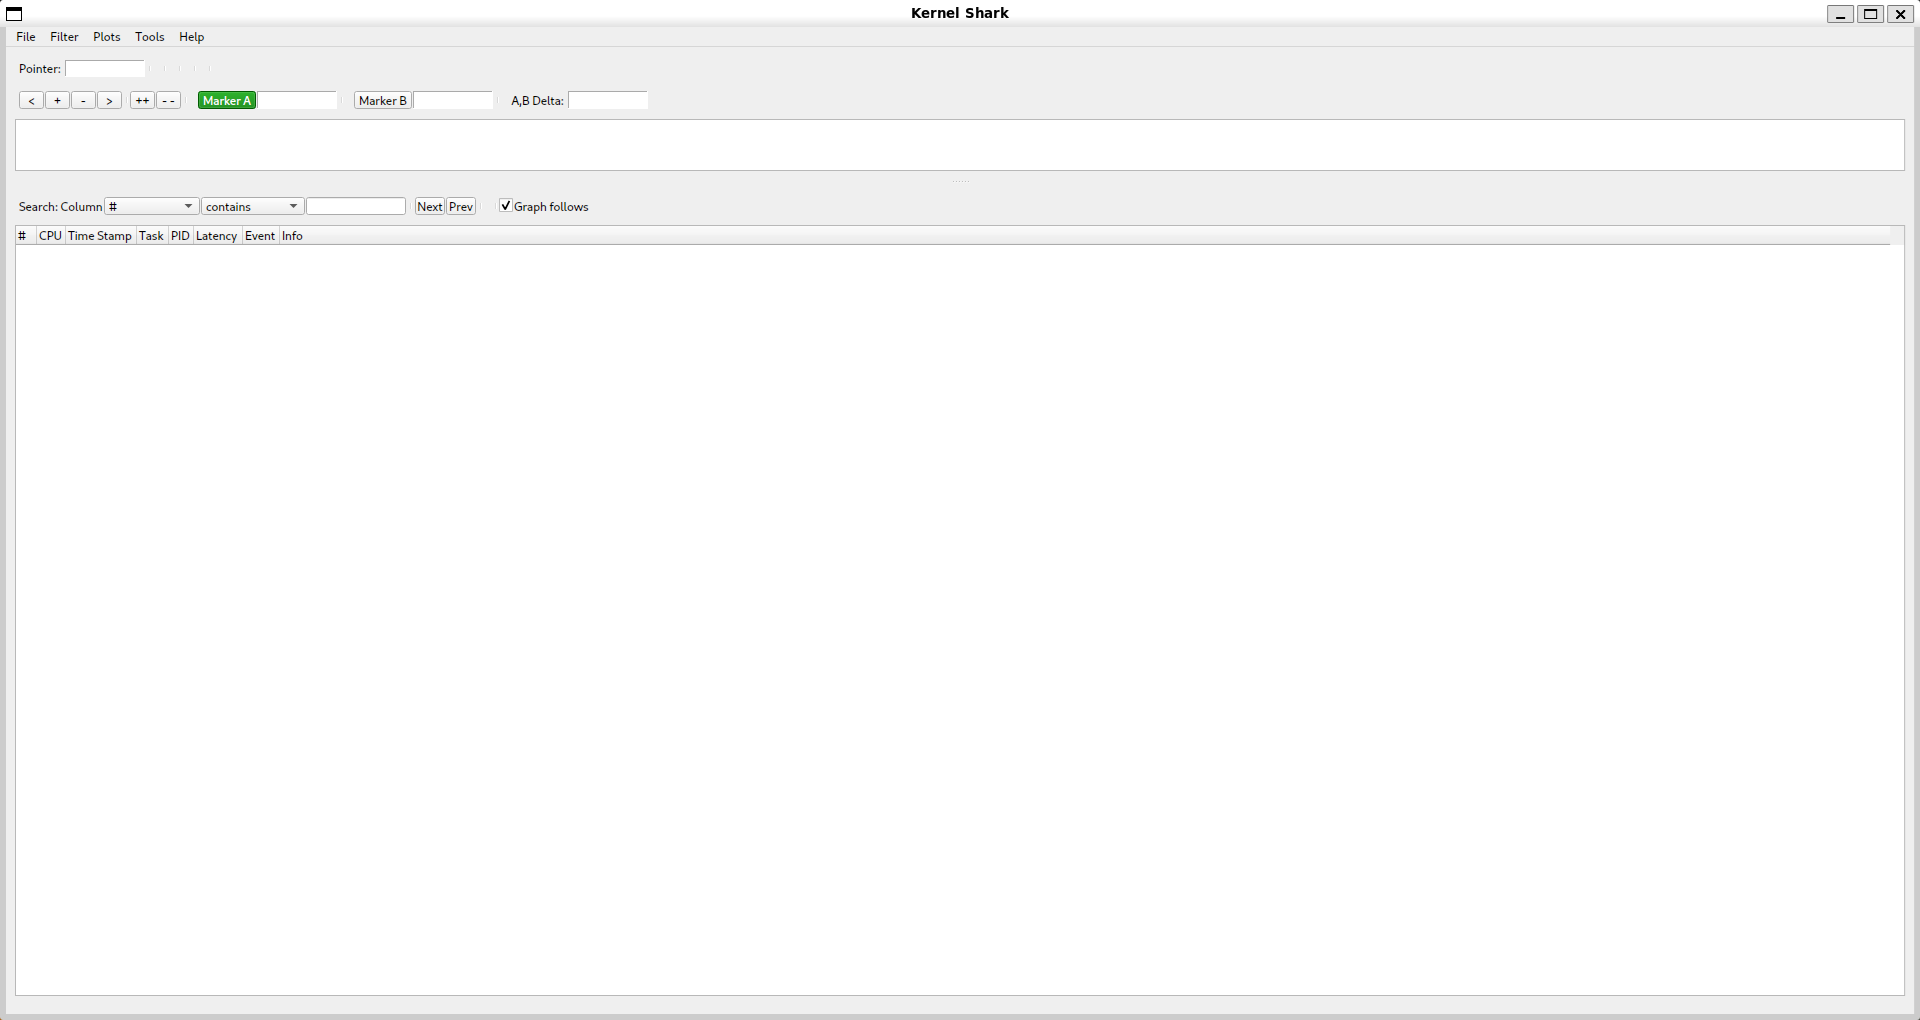
\includegraphics[width=140mm]{img/KernelShark/kshark-empty}
    \caption{Čerstvě spuštěný KernelShark}
    \label{kshark-empty}
\end{figure}

\subsection*{Hlavní okno}
Po spuštění se zobrazí hlavní grafické okno. To je rozdělené na 3 části: \emph{menu}, \emph{grafová oblast} a \emph{seznamová oblast}. Části jsou zvýrazněny na obrázku \ref{kshark-divs}, kde jsme KernelSharku dali nějaká data k zobrazení.

\begin{figure}[p]\centering
    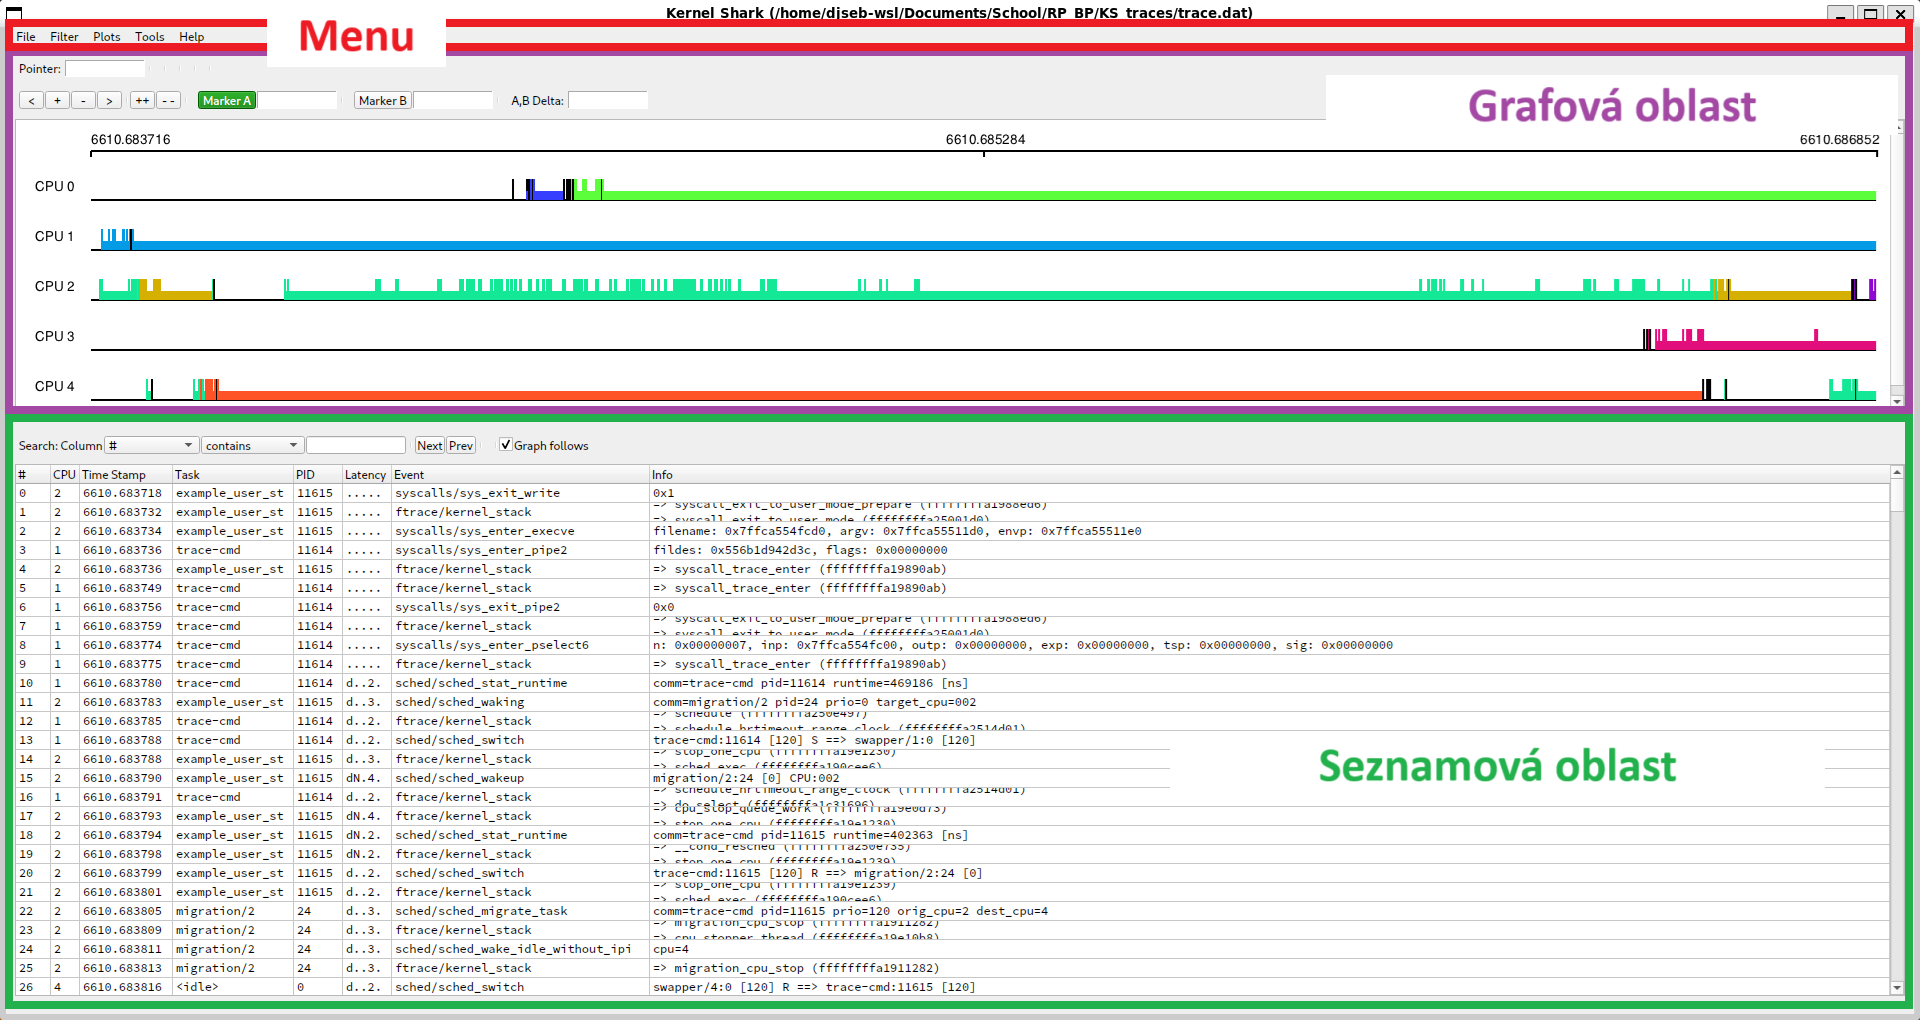
\includegraphics[width=140mm]{img/KernelShark/kshark-divisions}
    \caption{KernelShark se zvýrazněným dělením hlavního okna}
    \label{kshark-divs}
\end{figure}

\subsubsection*{Menu}
V menu je několik tlačítek pro práci se soubory, pro filtrování, tlačítko pro otevření dokumentace a tlačítko s různými nástroji. Zde se například zapínají a vypínají pluginy, nebo mění barvy používané KernelSharkem v grafech. 

\subsubsection*{Grafová oblast}
Grafová oblast obsahuje graf trasování, kontrolní řádek a informační řádek. Graf trasování se pak skládá z grafů pro jednotlivá CPU (zobrazeny jsou události jen z daného CPU) či procesy (zobrazeny jsou jen události daného procesu). Tyto grafy zobrazují události uspořádané v čase, který je reprezentován horziontální osou. Samotné grafy jsou v grafu trasování uspořádány svisle a lze použít posuvník k navigaci. V každém z grafů jsou události vyznačeny krátkými barevnými svislými čarami. Takovou čáru označuje KernelShark za \emph{bin}. Pro velké objemy trasovacích dat se do binů seskupují záznamy událostí. Dokud jsou biny \uv{stejné věci} za sebou, jsou mezi nimi i, o trochu nižší, obdélníky, které souvislou práci vyznačují - výjimkou je zde \uv{idle proces}, kdy CPU nepracuje a tyto obélníky se nekreslí. Termínem \uv{stejná věc} myslíme buď stejný proces v CPU grafech, nebo stejné CPU v grafech procesů. Pro zobrazení užších časových úseků lze v grafu přibližovat a oddalovat.

V kontrolním řádku se zobrazují ovládací prvky pro pohyb a přibližování v grafu a tlačítka s informacemi o (časových) pozicích dvou značkovacích čar, nazvanými \uv{Marker A} a \uv{Marker B}. Pokud dvakrát klikneme na bin v grafu, můžeme tak jedním z markerů vyznačit danou časovou pozici a záznam, který se na ní udál. Tím se i zapíše pozice markeru. Vybranou pozici můžeme zrušit kliknutím pravého tlačítka myši s kurzorem nad tlačítkem daného markeru. Pro vybírání mezi markery A a B stačí s levým tlačítkem myši kliknout na tlačítko daného z markerů. Vedle tlačítek markerů je i informace o jejich časovém rozdílu. Pokud jsou markery aktivní, pak přibližování se bude snažit přiblížit oblast jimi vyznačenou (pokud je aktivní jen jeden, pak bude středem přiblížení bude událost, na kterou marker ukazuje).

V informačním řádku se zobrazuje (časová) pozice kurzoru myši a informace při najetí myši přes biny v grafu. Tyto informace jsou také v seznamu událostí.

\subsubsection*{Seznamová oblast}
Seznamová oblast zobrazuje trasovací data ve formě svislého seznamu s několika sloupci:
\begin{itemize}
    \item Pozice události v datech
    \item Identifikátor CPU - číselný, používá označování jako operační systém.
    \item Časová značka události - v sekundách, s přesností na desetiny mikrosekund.
    \item Název procesu
    \item PID procesu
    \item Latence - jedná se o čtyři datová pole:
    \begin{itemize}
        \item Zdali byla vypnuta přerušení, označeno písmenem \uv{d}, jinak znakem \uv{.}.
        \item Zdali je potřeba přeplánování úloh, označeno písmenem \uv{N}, jinak znakem \uv{.}.
        \item Událost při vyřizování přerušení, písmeno \uv{h} značí přerušení od hardwaru, písmeno \uv{s} značí přerušení vyvolané kernelem či pokud je tento typ přerušení vypnutý, písmeno \uv{H} značí přerušení od hardwaru, kde jsou přerušení od kernelu vypnuta, nebo se hardwarové přerušení událo při obsluze vyrušení od kernelu - jiné situace jsou značeny znakem \uv{.}.
        \item Čítač preempce - pokud je jiný než 0, tak kernel nepřepíná běžící úlohy, i kdyby nějaké událost o přeplánování zažádala. Pokud je čítač nulový, zobrazí se znak \uv{.}.
    \end{itemize}
    \item Název události
    \item Dodatečné informace - data zaznamenána v dané události. 
\end{itemize}

V seznamu lze vyhledávat dle informací ve sloupcích, uživatel k tomu má dispozici textový vyhledávací řádek. V seznamu lze vyhledávat dopředu, či pozpátku. KernelShark podporuje jednoduchá vyhledávání typu \uv{obsahuje} (ve sloupci je někde vyhledávaný text), \uv{přesná shoda} (ve sloupci je pouze vyhledávaný text), \uv{neobsahuje} (ve sloupci není vyhledávaný text). Úspěšné vyhledávání v seznamu vyznačí událost splňující vyhledávací kritéria. Pokud je zaškrtnuté políčko \uv{Graph follows}, bude tato událost vyznačena i v grafu.

\subsection*{Filtrování}
Kvůli objemu dat získaných při trasování je často užitečné mít možnost ve vizualizaci filtrovat data, se kterými chceme při analýze pracovat. KernelShark proto dodává filtrovací nástroje - jednoduché filtry a pokročilé filtry. Jednoduché filtry filtrují podle typu události, zatímco pokročilé filtry dovolují vytvářet pokročilé filtrovací konstrukce a lze s nimi filtrovat i události dle jejich obsahu. KernelShark také dovoluje filtrovat události podle CPU nebo procesů. Pokud událost neprojde filtrem, pak není zobrazena v grafu ani v seznamu. Pokud na ni ukazoval nějaký marker, pak je vyznačen čárkovanou čarou. Jediné, co zůstane nepozměněno, jsou obdélníky mezi záznamy, které signalizují práci na CPU (graf CPU) nebo práci procesu (graf procesu).

K filtrům se lze dostat přes tlačítko \texttt{Filters} v menu. Všechny typy filtrování zobrazí uživateli dialog, přičemž filtrování podle typu události, CPU, nebo podle procesu zobrazí seznamy, kde se jednotlivé prvky k filtrování dají zaškrtnout a odškrtnout (tj. při filtrování podle CPU se zobrazí seznam CPU, při filtrování pole typu události se zobrazí seznam událostí). Speciiálně filtrování podle typu události ještě seskupuje události pod subsystémy, kterým patří, čímž je vytvořen dvouúrovňový seznam.

Pokročilé filtrování má dialog komplikovanější, přítomen je krátký pomocný text s příkladem použití, seznam aktivních pokročilých filtrů, soubor z něhož KernelShark čerpá data, pak tři řádky na sestavení filtru a nakonec filtr v textové podobě, kterou může uživatel upravovat. Zmíněné tři řádky na sestavení představují zjednodušení konstrukce filtru. První dovoluje vybrat událost z událostí přítomných v souboru s daty. Na druhé řáce může uživatel vybrat z \uv{operátorů}, nicméně lze si vybrat i čárky, závorky, speciální znaky pro regex a i skutečné operátory, které mohou být relační nebo boolovské. Třetí řádek zobrazuje datová pole z formátu události, která lze použít k filtrování, například pole \texttt{comm\_pid}, nebo speciálně pro událost sched\_switch pole \texttt{prev\_state}. Jednoduchý příklad pokročlého filtrování je na obrázku \ref{kshark-advfiltering}.

\begin{figure}[p]\centering
    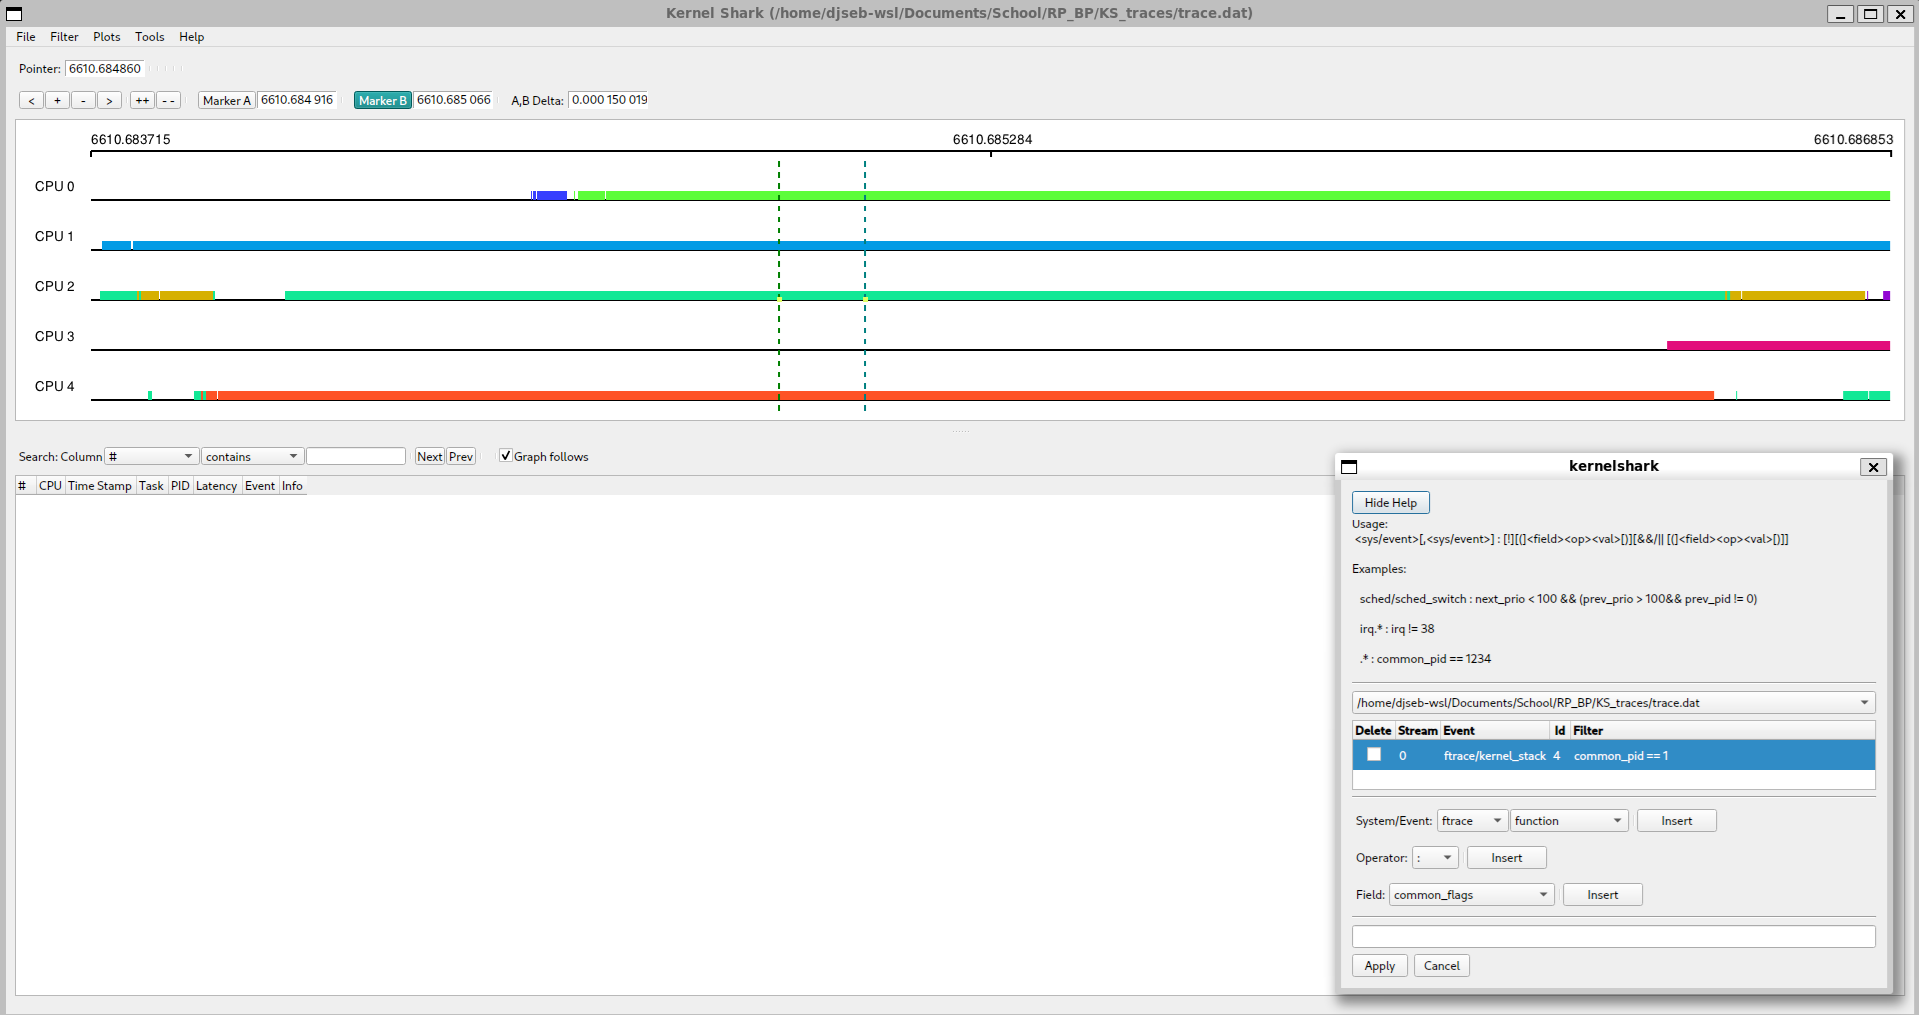
\includegraphics[width=140mm]{img/KernelShark/kshark-advfilter-in-effect}
    \caption{Aktivní pokročilý filtr - žádná událost nevyhovuje podmínkám}
    \label{kshark-advfiltering}
\end{figure}

\subsection*{Relace}
Při analýze si uživatel často vytvoří nějaký kontext k práci, například si vybere zajímavou oblast dat, vyznačí si nějakou událost Markerem B, načte si pluginy, nebo nějaké z nich povypíná a možná pracuje s více streamy naráz. Analýza také nemusí být záležitostí pár minut a uživatel může KernelShark vypnout během ní. Součástí KernelSharku jsou tedy i uživatelské relace, anglicky \uv{sessions}, do kterých se právě tato data ukládají. Relace se uloží do souboru a uživatel může začít od bodu posledního uložení relace. Ukládání je prováděno ručně, nic se neukládá automaticky. Samotné soubory jsou ve formátu JSON a je možné je manuálně upravovat. Speciálně u pluginů KernelShark kontroluje jejich verzi a plugin o novější či starší verzi, než jaká je uložena, nenačte.

\subsection*{Trace-cmd GUI}

KernelShark dovoluje uživateli sbírat data od Trace-cmd skrze GUI. Uživatel musí pouze kliknout na tlačítko \texttt{Record} v menu \texttt{Tools}. Poté program zažádá o superuživatelská oprávnění přes nějaký aktivní Polkit. Při úspěšné elevaci oprávnění KernelShark zobrazí nové okénko (viz obrázek \uv{Record okénka} \ref{kshark-record}). V něm je napravo plocha pro kontrolu běžícího Trace-cmd a nalevo jsou konfigurační možnosti trasování. V nich si uživatel může vybrat, které události chce zaznamenávat, jaký tracer má Trace-cmd použít, cestu k výstupnímu souboru, zdali si uživatel přeje vidět výstup a nakonec textové pole s příkazem, který spustí trasovaný proces (ve výchozím nastavení je zde pouze \texttt{sleep 0.1}). Do tohoto pole lze přiat i další argumenty pro spuštění Trace-cmd. Nakonec jsou dole v konfigurační ploše tři tlačítka. Jedním se toto okno zavře, druhým se aplikuje konfgurace a třetím se trasování spustí. Uživatel tak teoreticky s Trace-cmd vůbec nemusí pracovat v terminálu a může používat pouze KernelShark.

\begin{figure}[p]\centering
    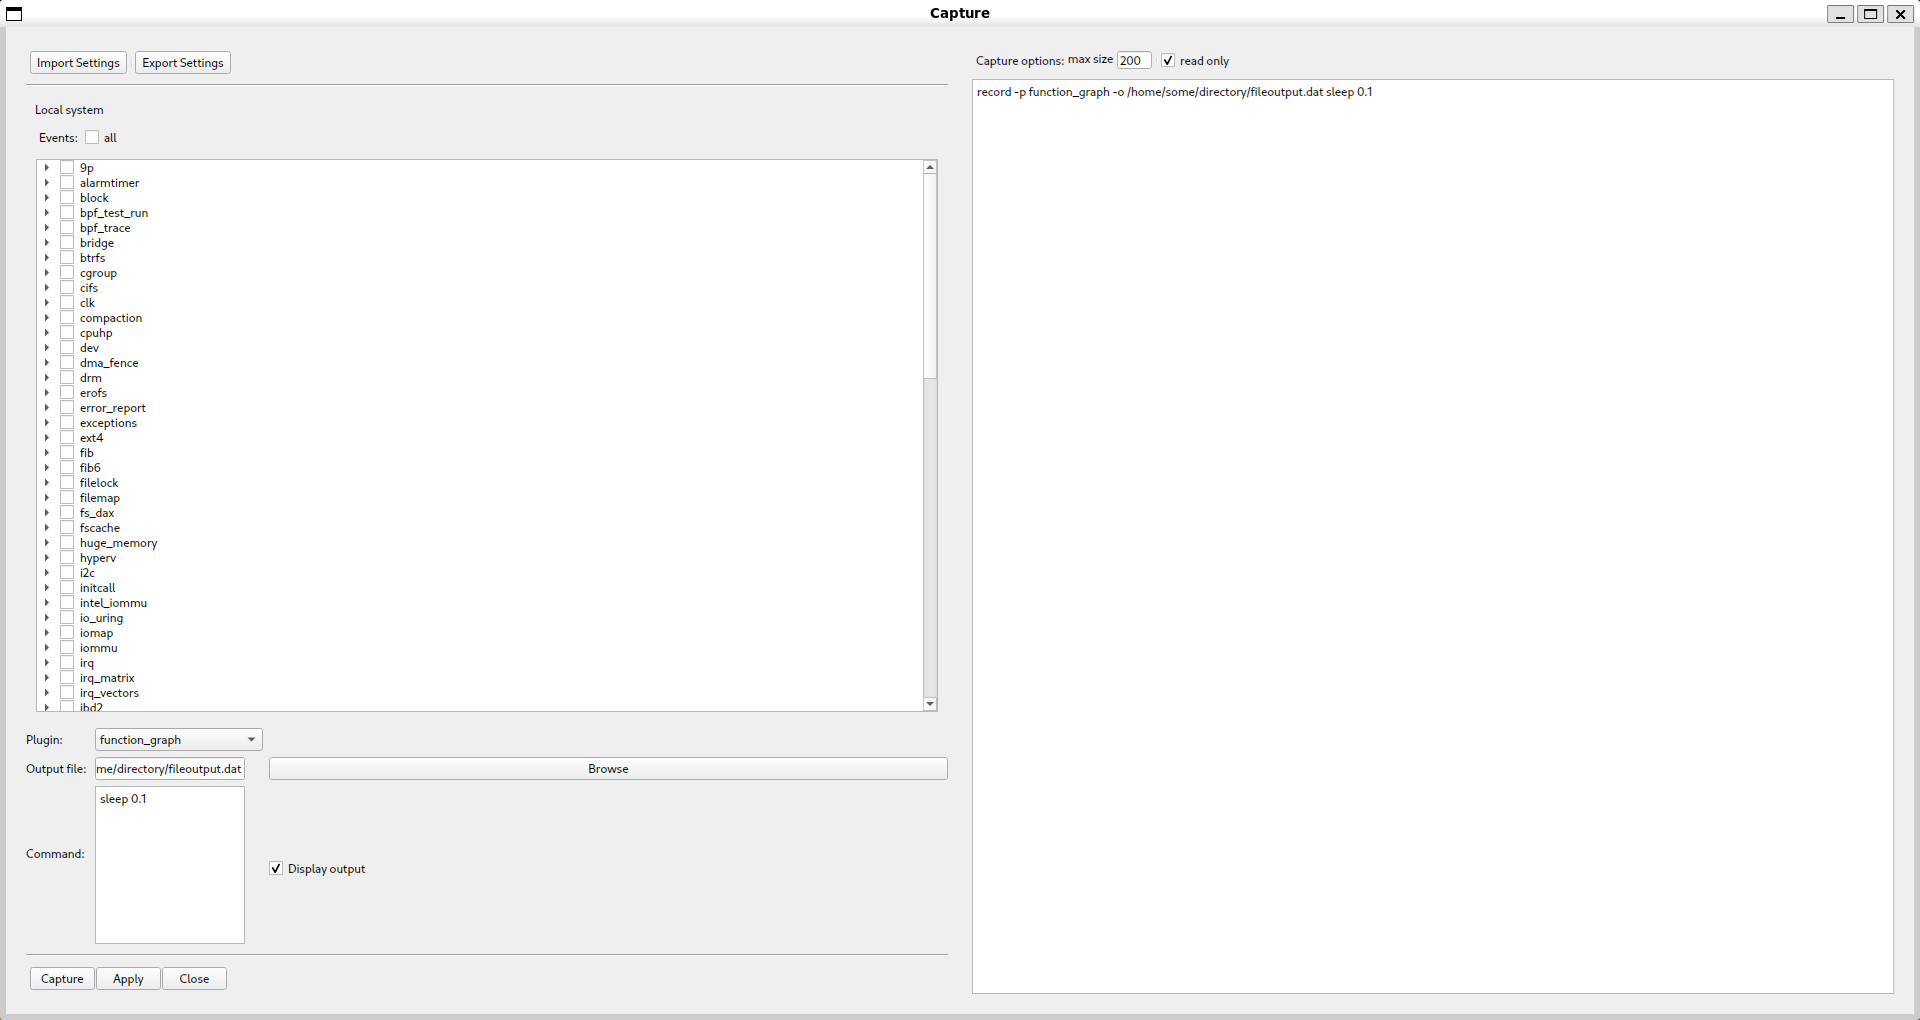
\includegraphics[width=140mm]{img/KernelShark/kshark-record}
    \caption{KernelShark GUI pro práci Trace-cmd}
    \label{kshark-record}
\end{figure}

\section{Pluginy}

KernelShark obsahuje rozhraní k vytváření pluginů, kterými pak může uživatel rozšířit chování programu, nejčastěji skrze kreslení do grafu či úpravu dat a nebo sběr statistik. KernelShark dovoluje vývojářům pluginů definovat menu pro pluginy, jejich chování při načítání trasovacích dat a kreslení aktivního pluginu. Uživatel může i nemusí využít všechny tyto možnosti. KernelShark také obsahuje některé pluginy ve svojí základní instalaci, které označíme v této práci jako \emph{oficální pluginy}. Mezi tyto pluginy patří například plugin sched\_events, který kreslí červené a zelené rámečky do grafů procesů. Oficiální pluginy také představují inspiraci pro vývojáře dalších pluginů.

Obecně pluginy definují kontext, tj. jejich vlastní \uv{globální úložiště}, jejich inicializační a deinicializační funkce, a handlery právě pro kreslení, či úpravu dat při načítání a nebo pro vytvoření menu. Vše ostatní je pak na vývojáři pluginu. KernelShark obsahuje speciální sestavovací instrukce pro pluginy, přičemž je možné dát zdrojové soubory vlastních pluginů do adresáře se zdrojovými soubory oficálních pluginů a upravit tyto instrukce. Pokud si ale vytvoříme sestavovací instrukce sami, KernelShark stále plugin přijme.

\section{Architektura programu}

Následující sekce bude autorův pokus o zachycení architektury KernelSharku. Architektura nemá vlastní dokumentaci, tato sekce tak nemůže zaručit, že architektura nastíněná zde je perfektním odrazem architektury ve vizi autorů KernelSharku. Nicméně se nám tento odhad bude hodit pro orientaci v kódu programu v této práci.

Obecně lze říci, že KernelShark je grafická aplikace, která používá klasický přístup zachytávání událostí uživatelské interakce ve smyčce a jejich následné zpracování. Má nějaký hlavní systém a k němu jsou definována místa pro práce pluginů.

Detailnější pohled na architekturu zachytíme pomocí modulů. Nebdeme se zaměřovat na konkrétní implementace.
\begin{itemize}
    \item \emph{Zpracovávání dat} - zde se KernelShark zaměřuje hlavně na čtení dat a jejich abstrakce, které KernelShark používá dále. Velkým zaměřením je transformace dat z Trace-cmd do lépe vizualizovatelných dat. Právě zde nejvíce žijí streamy a záznamy KernelSharku. Součástí jsou i dotazy na data v záznamech či ve streamech.
    % libkshark + libkshark-tepdata + libkshark-hash
    \item \emph{Datové modely} - KernelShark pracuje s několika datovými modely podle potřeby. Základním modelem jsou prvky uspořádané dle času do binů, tj. sdružení záznamů. S tímto modelem KernelShark pracuje nejvíce a dodává k němu i API na manipulaci a dotazování, například na index (do pole všech záznamů) prvního záznamu v daném binu. Existují ale i modely vhodnější pro seznamové zobrazení událostí a model pro filtrování takových seznamů.
    % KsModels + libkshark-model 
    \item \emph{Trace-cmd GUI} - modul starající se o vše týkající se okna pro práci s Trace-cmd skrze KernelShark.
    % KsCaptureDialog + kshark-record
    \item \emph{Hlavní okno} - zde se seskupují hlavní grafické prvky, tj. graf trasování, seznam událostí a menu programu. Toto okno také představuje hlavní navigovatelný prvek v kódu, přes který se lze dostat k dalším (veřejným) prvkům, třeba právě ke grafu trasování a jeho prvkům.
    % KsMainWindow + kernelshark + % KsTraceViewer + % KsDualMarker + KsGLWidget + KsTraceGraph
    \item \emph{Kreslení v grafu} - aby bylo možné kreslit do grafu, dodává KernelShark několik definic tvarů, jejich kreslení a interakce s myší (pouze dvojité kliknutí) v tomto modulu. Tyto tvary jsou pak nejvíce využívány pluginy při vytváření tvarů vlastních.
    % KsPlotTools + libkshark-plot + KsPlugins
    \item \emph{Filtry} - modul se stará o vše ohledně filtrování, ať už filtrování samotné, vyhledávání správných událostí, nebo okna, se kterými uživatel pracuje při filtrování.
    % KsAdvancedFilteringDialog + libkshark 
    \item \emph{Vyhledávání} - modul se stará o vyhledávání v seznamu událostí, ale i vyhledávání uskutečněná nějakým kódem.
    % KsSearchFSM + libkshark-collections.c + libkshark
    \item \emph{Relace} - zde najdeme \uv{ukládací} a \uv{načítací} funkce pro všechno, co KernelShark do relací ukládá.
    % KsSession + libkshark-configio.c + libkshark
    \item \emph{Pluginy} - tento modul se stará hlavně o načítání, zapínání, inicializaci a působení pluginů (tj. kde se volají jejich handlery). Dodává i některé definice a deklarace, které mohou pluginy využít.
    % KsPlugins + KsPluginsGUI + libkshark-plugin + ofiko pluginy
    \item \emph{Pomocné nástroje} - modul s různými funkcemi a strukturami, kterými si KernelShark pomáhá. Patří sem definice některých vyskakovacích oken, funkce na získání užitečných dat, například všech CPU ve streamu, nebo operátory pro práci s barvami.
    % KsUtils + KsWidgetsLib + KsQuickContextMenu
\end{itemize}